\documentclass[10pt,a4paper]{report}
%\usepackage[latin1]{inputenc}
\usepackage[utf8]{inputenc}
\usepackage{amsmath}
\usepackage{amsfonts}
\usepackage{amssymb}
\usepackage{graphicx}
\usepackage{multicol}
\usepackage{tabularx}
\usepackage{tikz}
\usetikzlibrary{arrows,shapes,automata,petri,positioning,calc}
\usepackage{hyperref}
\usepackage{tikz}
\usetikzlibrary{matrix,calc}
\usepackage[margin=0.5in]{geometry}
% ---- power functions -----% 
\newcommand{\myvec}[1]{\ensuremath{\begin{pmatrix}#1\end{pmatrix}}}
\let\vec\mathbf

\providecommand{\norm}[1]{\left\lVert#1\right\rVert}
\providecommand{\abs}[1]{\left\vert#1\right\vert}
\let\vec\mathbf

\newcommand{\mydet}[1]{\ensuremath{\begin{vmatrix}#1\end{vmatrix}}}
\providecommand{\brak}[1]{\ensuremath{\left(#1\right)}}
\providecommand{\lbrak}[1]{\ensuremath{\left(#1\right.}}
\providecommand{\rbrak}[1]{\ensuremath{\left.#1\right)}}
\providecommand{\sbrak}[1]{\ensuremath{{}\left[#1\right]}}
%-------end power functions----%
\newenvironment{Figure}
  {\par\medskip\noindent\minipage{\linewidth}}
  {\endminipage\par\medskip}
\begin{document}
%--------------------logo figure-------------------------%
\begin{figure*}[!tbp]
  \centering
  \begin{minipage}[b]{0.4\textwidth}
    
\includegraphics[scale = 0.05]{iitlogo.jpg}
  \end{minipage}
  \hfill
  \vspace{5mm}\begin{minipage}[b]{0.4\textwidth}
\raggedleft  
\includegraphics[scale = 0.10]{nrc.png}\

  \end{minipage}\vspace{0.2cm}
\end{figure*}
%--------------------name & rollno-----------------------
\raggedright \textbf{Name}:\hspace{1mm} D. Siva Krishna\hspace{3cm} \Large \textbf{Assignment-4}\hspace{2.5cm} % 
\normalsize \textbf{Roll No.} :\hspace{1mm} FWC22065\vspace{1cm}
\begin{multicols}{2}

%----------------problem statement--------------%
\raggedright \textbf{Problem Statement:}\vspace{2mm}
\raggedright \\The slope of a line is double of the slope of another line. If tangent of the angle between them is 1/3, find the slopes of the lines.\\
\vspace{5mm}
%-----------------------------solution---------------------------
\raggedright \textbf{SOLUTION}:\vspace{2mm}\\

%---------given----------------%
\raggedright \textbf{Given}:\vspace{2mm}\\
Slope of one line is double of the slope of the other line. \\\vspace{1mm}
The direction vector of a line is expressed as
\\
\begin{align}
\vec{m}=\myvec{1\\m}
\end{align}
where  m is defined to be the slope of the line.\\
\vspace{2mm}
 Also given that the tangent of the angle between them is $\frac{1}{3}$.   \\
\begin{align}
\tan \theta = \frac{1}{3}\\
\vspace{2mm}
\\
\implies \cos \theta=\frac{3}{\sqrt{10}}
\end{align}
\\
%--------------steps----------------------%
\textbf{Input Parameters:}
\vspace{2mm}


\begin{tabular}{|c|c|c|}
	\hline
	\textbf{Symbol}&\textbf{Value}&\textbf{Description}\\
	\hline
	$\vec{m_1}$ &\myvec{1\\m}& Direction vector\\
	\hline
    $\vec{m_2}$ &\myvec{1\\2m}&Direction vector\\
	\hline
    $\tan\theta$ &1/3& Angle\\
	\hline
\end{tabular}
\\
\vspace{10cm}
The angle between two vectors is expressed as
\\ \vspace{1mm}
\begin{align}
\cos \theta = \frac{{\textbf{A}}^\top \textbf{B}}{\norm{\textbf{A}}\norm{\textbf{B}}}
\end{align} 
%Substituting the \vec{m_1} and \vec{m_2} in the above equation
\\
\begin{align}
\frac{3}{\sqrt{10}} = \frac{\vec{m_1}^\top \vec{m_2}}{\norm{\vec{m_1}}\norm{\vec{m_2}}}
\\
\\
\frac{3}{\sqrt{10}} = \frac{\myvec{1 \hspace{2mm} m}\myvec{1 \\ 2m}}{\norm{\myvec{1\\m}}\norm{\myvec{1\\2m}}}
\\
\\
\frac{3}{\sqrt{10}} = \frac{2m^2 +1}{\sqrt{m^2 + 1}\sqrt{4m^2 + 1}}
\end{align}
\vspace{2mm}
Squaring on both sides,
\begin{align}
\frac{9}{10}=\frac{4m^4 + 4m^2 +1}{4m^4 + 5m^2 +1}
\\
\\
4m^4 - 5m^2 +1 = 0
\end{align}
Let $m^2$ = x and substituting it in above equation we get a quadratic equation.
\begin{align}
	4x^2 -5x +1 = 0
\end{align}
From the formula of fining roots of a quadratic equation
\begin{align}
	\frac{-b\pm \sqrt{b^2 - 4ac}}{2a}
	\\
	\\
	\frac{5\pm \sqrt{\left (-5\right )^2 - 16}}{8}
	\\
	x= 1 (or) x = 1/4
\end{align}
\\
The slope of the first line is
\\
\begin{center}
$ \therefore m=\pm \frac{1}{2}$\\
    (or)\\
    $m=\pm 1$
\end{center}
$\therefore $ Slope of second line is
\begin{center}
$ 2m=\pm 1$\\
    (or)\\
    $2m=\pm 2$
\end{center}
\begin{center}
 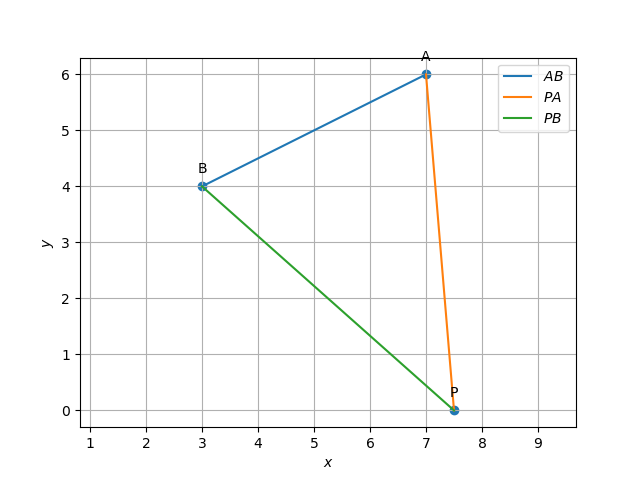
\includegraphics[width=0.5\textwidth]{line.png}  
 \end{center}\vspace{1mm}
\raggedright  Download the code \\
Github link:{Assignment-4}.
\end{multicols}
\end{document}
